\documentclass[border=4pt]{standalone}
\usepackage[T1]{fontenc}
\usepackage{helvet}
\renewcommand{\familydefault}{\sfdefault}
\usepackage{tikz}
\usetikzlibrary{arrows.meta,positioning,fit,backgrounds,shapes.geometric,calc}
\definecolor{ink}{HTML}{1F3A56}
\definecolor{core}{HTML}{DCE7F2}
\definecolor{know}{HTML}{DDEFE8}
\definecolor{game}{HTML}{F6E8D6}
\definecolor{model}{HTML}{EAE3F3}
\definecolor{plain}{HTML}{F3F4F6}
\definecolor{bad}{HTML}{B3402E}
\tikzset{
 every node/.style={font=\fontsize{8.5}{10.2}\selectfont,align=center,text=ink,execute at begin node={\hyphenpenalty=10000\exhyphenpenalty=10000}},
 box/.style={draw=ink,fill=white,rounded corners=1.5pt,minimum height=8.5mm,inner sep=3pt,line width=.5pt},
 corebox/.style={box,fill=core},
 knowbox/.style={box,fill=know},
 gamebox/.style={box,fill=game},
 modelbox/.style={box,fill=model},
 plainbox/.style={box,fill=plain},
 planned/.style={dashed},
 flow/.style={-{Stealth[length=2mm]},draw=ink,line width=.6pt},
 dflow/.style={flow,dashed},
 badflow/.style={flow,draw=bad,dashed},
 band/.style={draw=ink!55,rounded corners=3pt,inner sep=6pt,line width=.45pt},
 title/.style={font=\bfseries\fontsize{8.5}{10.2}\selectfont},
 lab/.style={font=\fontsize{7.5}{9}\selectfont,fill=white,inner sep=1pt},
 decision/.style={diamond,draw=ink,fill=core,aspect=2.1,inner sep=0.5pt,line width=.5pt}
}

\begin{document}
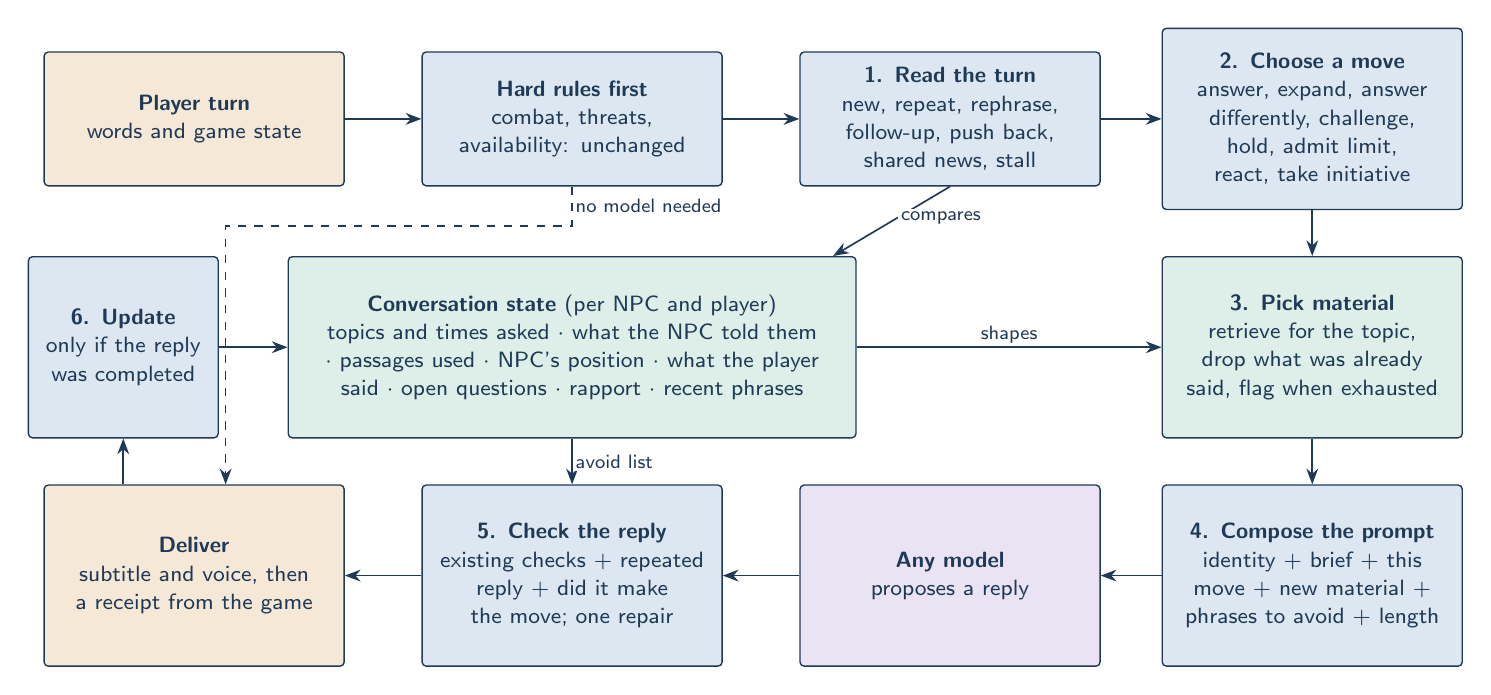
\begin{tikzpicture}[x=1mm,y=1mm]
\def\tw{36mm}
% Top row: the turn, left to right.
\node[gamebox,text width=\tw,minimum height=17mm] (in) at (20,62) {\textbf{Player turn}\\words and game state};
\node[corebox,text width=\tw,minimum height=17mm] (rules) at (68,62) {\textbf{Hard rules first}\\combat, threats, availability: unchanged};
\node[corebox,text width=\tw,minimum height=17mm] (act) at (116,62) {\textbf{1. Read the turn}\\new, repeat, rephrase, follow-up, push back, shared news, stall};
% Middle row: the state in the centre.
\node[knowbox,text width=70mm,minimum height=23mm] (state) at (68,33) {\textbf{Conversation state} (per NPC and player)\\topics and times asked $\cdot$ what the NPC told them $\cdot$ passages used $\cdot$ NPC's position $\cdot$ what the player said $\cdot$ open questions $\cdot$ rapport $\cdot$ recent phrases};
\node[corebox,text width=\tw,minimum height=23mm] (move) at (162,62) {\textbf{2. Choose a move}\\answer, expand, answer differently, challenge, hold, admit limit, react, take initiative};
\node[knowbox,text width=\tw,minimum height=23mm] (material) at (162,33) {\textbf{3. Pick material}\\retrieve for the topic, drop what was already said, flag when exhausted};
% Bottom row: right to left.
\node[corebox,text width=\tw,minimum height=23mm] (prompt) at (162,4) {\textbf{4. Compose the prompt}\\identity + brief + this move + new material + phrases to avoid + length};
\node[modelbox,text width=\tw,minimum height=23mm] (model) at (116,4) {\textbf{Any model}\\proposes a reply};
\node[corebox,text width=\tw,minimum height=23mm] (check) at (68,4) {\textbf{5. Check the reply}\\existing checks + repeated reply + did it make the move; one repair};
\node[gamebox,text width=\tw,minimum height=23mm] (deliver) at (20,4) {\textbf{Deliver}\\subtitle and voice, then a receipt from the game};
\node[corebox,text width=22mm,minimum height=23mm] (update) at (11,33) {\textbf{6. Update}\\only if the reply was completed};
\draw[flow] (in) -- (rules);
\draw[flow] (rules) -- (act);
\draw[flow] (act) -- (move);
\draw[flow] (act.south) -- node[lab,right,pos=.45] {compares} ($(state.north east)+(-3,0)$ |- state.north);
\draw[flow] (move) -- (material);
\draw[flow] (material) -- (prompt);
\draw[flow] (prompt) -- (model);
\draw[flow] (model) -- (check);
\draw[flow] (check) -- (deliver);
\draw[flow] (deliver.north -| update) -- (update);
\draw[flow] (update) -- (state);
\draw[flow] (state.east) -- node[lab,above] {shapes} (material.west);
\draw[flow] (state.south -| check) -- node[lab,right] {avoid list} (check.north);
\draw[dflow] (rules.south) -- ++(0,-5) node[lab,right,pos=.5] {no model needed} -| ($(deliver.north)+(4,0)$);
\end{tikzpicture}
\end{document}
